\documentclass{article}
\usepackage[utf8]{inputenc}
\usepackage[spanish]{babel}
\usepackage[letterpaper, portrait, margin=2cm]{geometry}
\usepackage[style=ieee]{biblatex}
\usepackage{amsthm}
\usepackage{amsmath}
\usepackage{amssymb}
\usepackage{amsfonts}
\usepackage{hyperref}
\usepackage{csquotes}
\usepackage{mathtools}
\usepackage{graphicx}
\usepackage{float}
\usepackage{array}
\usepackage{dirtytalk}
\usepackage[table,xcdraw]{xcolor}

\usepackage{listings}

\DeclarePairedDelimiter{\ceil}{\lceil}{\rceil}

\definecolor{codegreen}{rgb}{0,0.6,0}
\definecolor{codegray}{rgb}{0.5,0.5,0.5}
\definecolor{codepurple}{rgb}{0.58,0,0.82}
\definecolor{backcolour}{rgb}{0.95,0.95,0.92}

\lstdefinestyle{mystyle}{
    backgroundcolor=\color{backcolour},   
    commentstyle=\color{codegreen},
    keywordstyle=\color{magenta},
    numberstyle=\tiny\color{codegray},
    stringstyle=\color{codepurple},
    basicstyle=\ttfamily\footnotesize,
    breakatwhitespace=false,         
    breaklines=true,                 
    captionpos=b,                    
    keepspaces=true,                 
    numbers=left,                    
    numbersep=5pt,                  
    showspaces=false,                
    showstringspaces=false,
    showtabs=false,                  
    tabsize=2
}

\lstset{style=mystyle}

\title{Anexos de Investigación: Modelo de Muestreo Virtual de Suelos Agrícolas en Honduras para Analítica en Base al Muestreo Aleatorio Simple y Estratificado}
\author{Tobias Briones \bigbreak tobias.briones@unah.hn}
\date{Diciembre 2021}

\begin{document}

\makeatletter
    \begin{titlepage}
        \begin{center}
            
\includegraphics[width=0.3\linewidth]{ref/logo-unah.png}\\[4ex]
            {\huge \bfseries \@title 
            \vspace{1cm}}\\[2ex]
            {\LARGE \@author}\\[50ex] 
            
            {\large
            Proyecto de Seminario de Investigación Presentado a la\\
            Universidad Nacional Autónoma de Honduras de la Carrera de\\
            Licenciatura en Matemática
            }\\[2ex]
            
            {\large \@date}
        \end{center}
    \end{titlepage}
\makeatother
\thispagestyle{empty}
\newpage

\section{Anexos}

\subsection{Introducción}

\begin{lstlisting}[language=Python, caption=Introducción al enunciados del problema (Hoja 1)]
from main import plot
from test import hn_example as hn

# ----------

hn_gis = hn.Gis()

hn_gis.parent_dir = './test'

# ----------

# SIG

hn_gdf = hn_gis.load()
hn_df = hn_gis.df()

hn_df

# ----------

# Muestreo fisico (generado aleatoriamente)

hard_sampling = hn.HardSampling.generate()

hard_sampling

# ----------

# SIG

plot(hn_gdf, 'Mapa de Suelo Agricola por Lotes', size=20)

# Mapa de Suelo Agricola por Estratos
hn_gdf.plot(figsize=(20, 20), column=hn.STRATUM_COL, legend=True)

# ----------

from test import main
import sampling

main = main.Main.new_instance('./test')
sampling = sampling.Sampling.from_main(main)
sim = sampling.new_sampling_simulator()

sampling.stratum_sampling_size(300)

sim.simulate(hn.Stratum.CP_72_2086)
\end{lstlisting}

\begin{figure}[H]
    \centering
    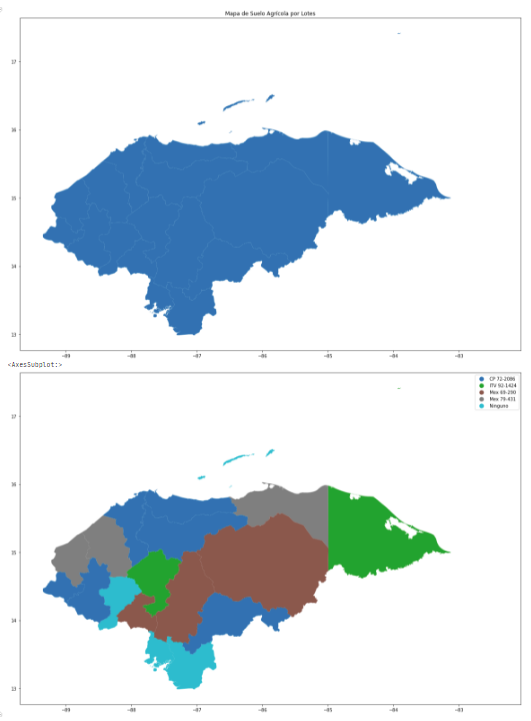
\includegraphics[width=0.5\paperwidth]{ref/intro-fig-1.png}
    \caption{Mapa del suelo agrícola}
    Fuente: Derivado de GADM data (version 3.6) \cite{gadm-2021}
\end{figure}

\begin{figure}[H]
    \centering
    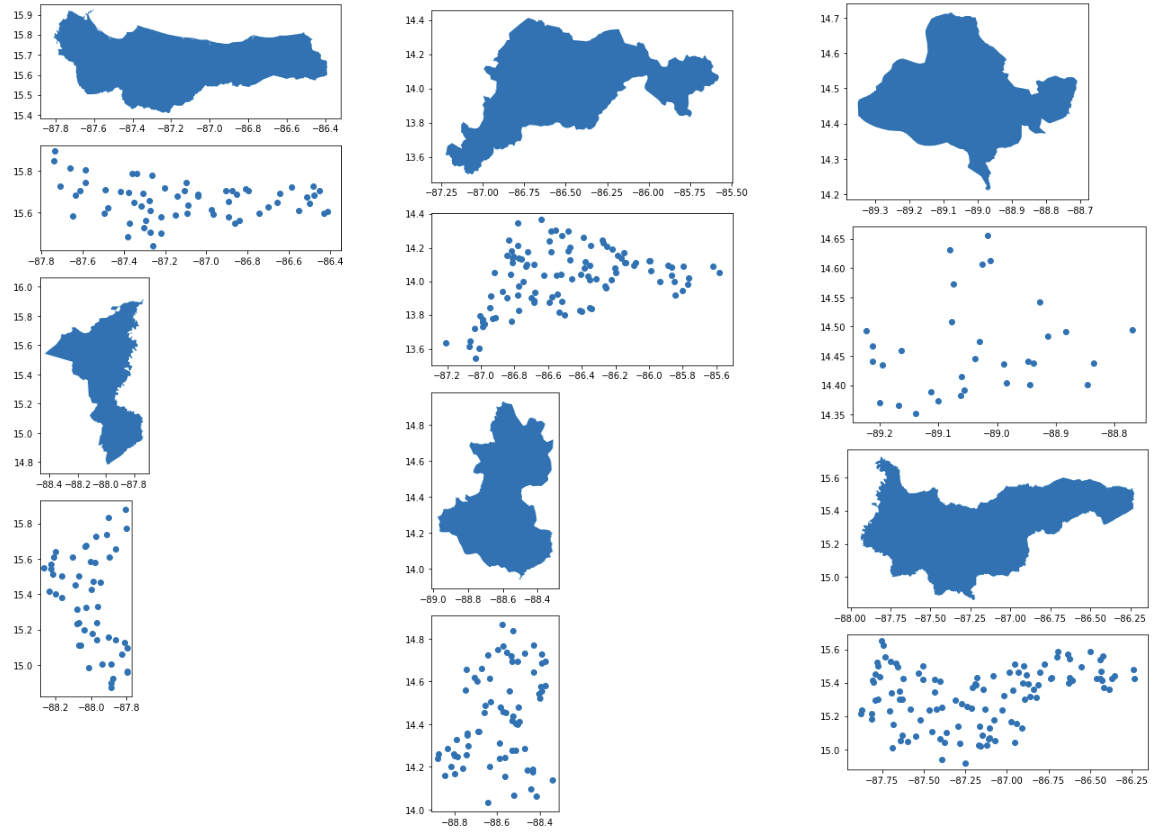
\includegraphics[width=0.3\paperwidth]{ref/intro-fig-2.png}
    \caption{Simulación de muestreo virtual para el estrato $CP \,\, 72-2086$}
    Fuente: Derivado de GADM data (version 3.6) \cite{gadm-2021}
\end{figure}

\end{document}
